\chapter{Resultados e Discussão} \label{chap:results}

\section{Refinamento de Malha}

Iniciamos nossa análise dos resultados com um estudo sobre o refinamento das malhas temporal e espacial. O objetivo é compreender como os resultados se comportam diante de variações nesses parâmetros, ou seja, a estabilidade da solução e, consequentemente, determinar o número de pontos na malha numérica para utilização.

De acordo com \citet{schiesser2009}, o ajuste do espaçamento da grade em diferentes partes ou em todo o domínio do problema é conhecido como refinamento "h". Essa nomenclatura é comumente usada na literatura de análise numérica, onde "h" é símbolo para o espaçamento da grade. O refinamento "h" busca melhorar a precisão da solução, refinando o espaçamento da grade com base em estimativas de erro de truncamento local ou outros parâmetros de refinamento. É importante destacar que não existe uma única combinação universalmente ideal de refinamento; a solução de problemas complexos frequentemente envolve tentativa e erro para encontrar o equilíbrio entre precisão e carga computacional. O objetivo final é alcançar um limite predefinido para o erro global com o mínimo esforço computacional necessário.

\subsection{Malha Temporal}

Para a presente análise, buscou-se analisar o máximo erro absoluto de uma malha com a equivalente mais refinada, a fim de se compreender a estabilidade das mesmas.

\begin{gather}
    \epsilon = \max | \Delta \theta | = \max | \theta(r,t_{n+1}) - \theta(r,t_{n}) |
\end{gather}

Através do estudo do refinamento da malha temporal, pode-se observar que, para malhas com até 1.281 pontos, não foram identificados erros significativos, como registrado na Tabela \ref{tab:error_in_the_temporal_mesh}. Quando o número de pontos variou de 1.281 para 20.481, observou-se uma discrepância praticamente insignificante.

No entanto, é importante destacar que, para malhas com mais de 40.961 pontos, o erro passou a ser significativo. Essa discrepância pode ser atribuída à formação de singularidades resultantes de um refinamento excessivo da malha em conjunto à tolerância de erro absoluto e/ou relativo predefinida no solver utilizado.

Portanto, optou-se por utilizar uma malha temporal com 100 pontos, que se mostrou apropriada para a resolução do problema em questão.

\begin{table}[H]
    \centering
    \caption{Erro numérico no refino da malha temporal.}
    \begin{tabular}{ccc}
        \textbf{Pontos na Malha} & \textbf{Tamanho da Malha {[}s{]}} & \textbf{Erro} \\ \hline
        11                       & 0,15                                          & -             \\
        21                       & 0,075                                         & 0             \\
        41                       & 0,0375                                        & 0             \\
        81                       & 0,0188                                        & 0             \\
        161                      & 0,00938                                       & 0             \\
        321                      & 0,00469                                       & 0             \\
        641                      & 0,00234                                       & 0             \\
        1.281                     & 0,00117                                       & 0             \\
        2.561                     & 5,86E-04                                      & 1,26E-12      \\
        5.121                     & 2,93E-04                                      & 9,66E-13      \\
        10.241                    & 1,46E-04                                      & 5,50E-12      \\
        20.481                    & 7,32E-05                                      & 3,94E-12      \\
        40.961                    & 3,66E-05                                      & 0,000519651  
    \end{tabular}
    \source{Autor, 2023.}
    \label{tab:error_in_the_temporal_mesh}
\end{table}

%Para mais detalhes, o Apêndice \ref{att:temporal_mesh_convergence_tables} apresenta os resultados do refino de malha temporal através de tabelas de convergência.

\subsection{Malha Espacial}

%Através do estudo do refinamento da malha espacial, constatou-se que o solver não é capaz de gerar resultados para malhas contendo menos de 76 pontos, gerando o seguinte erro: "Incapaz de atender às tolerâncias de integração sem reduzir o tamanho do passo abaixo do menor valor permitido (2,775558e-17) no tempo t."

Para a presente análise, buscou-se analisar o máximo erro absoluto de uma malha com a equivalente mais refinada, a fim de se compreender a estabilidade das mesmas.

\begin{gather}
    \epsilon = \max | \Delta \theta | = \max | \theta(r_{n+1},t) - \theta(r_{n},t) |
\end{gather}

Através do estudo do refinamento da malha temporal, pode-se observar que, para malhas com um número de pontos variando de 76 a 151, não foram observados erros significativos, como registrado na Tabela \ref{tab:error_in_the_spatial_mesh}. Quando o número de pontos variou de 151 para 2.401, observou-se uma discrepância praticamente insignificante.

No entanto, é importante destacar que, para malhas com mais de 2.401 pontos, o erro passou a ser significativo. Novamente, essa discrepância pode ser atribuída à formação de singularidades resultantes de um refinamento excessivo da malha em conjunto à tolerância de erro absoluto e/ou relativo predefinida no solver utilizado.

Portanto, optou-se por utilizar uma malha espacial com 100 pontos, que se mostrou apropriada para a resolução do problema em questão.

\begin{table}[H]
    \centering
    \caption{Erro numérico no refino da malha espacial.}
    \begin{tabular}{ccc}
        \textbf{Pontos na   Malha} & \textbf{Tamanho da Malha} & \textbf{Erro} \\ \hline
        76                         & 0,0133                    & -             \\
        151                        & 0,00667                   & 0             \\
        301                        & 0,00333                   & 3,51E-05      \\
        601                        & 0,00167                   & 1,14E-05      \\
        1.201                      & 8,33E-04                  & 2,19E-05      \\
        2.401                      & 4,17E-04                  & 1,18E-05      \\
        4.801                      & 2,08E-04                  & 0,00021       \\
        9.601                      & 1,04E-04                  & 0,00046      
    \end{tabular}
    \source{Autor, 2023.}
    \label{tab:error_in_the_spatial_mesh}
\end{table}

%Para mais detalhes, o Apêndice \ref{att:spatial_mesh_convergence_tables} apresenta os resultados do refino de malha espacial através de tabelas de convergência.

\section{Perfis de Transferência de Calor}

Nesta seção, discutiremos os resultados obtidos para quatro formas de geração de calor. Além disso, faremos uma comparação com os resultados apresentados por \citet{soares2017}, que por sua vez se baseou no trabalho de \citet{bhattacharya2001}. É relevante mencionar que os resultados de \citet{soares2017} foram obtidos digitalmente, utilizando um software para coletar pontos em curvas. Portanto, devemos considerar que alguns erros foram introduzidos durante esse processo.

Para todos os casos, inicialmente o valor do termo fonte de calor uniforme adimensional (\(G ^*\)) foi considerado igual a \(32,4\) e o número de \textit{Biot} foi considerado igual a \(15\), ambos seguindo a literatura.

\subsection{Primeira Forma de Geração de Calor}

A primeira forma de geração de calor foi proposta por \citet{bhattacharya2001} e referenciada por \citet{soares2017}, ela se dá pela equação:

\begin{gather}
    G ' = G ^* t
    \label{eq:first_form_of_heat}
\end{gather}

\begin{figure}[H]
    \centering
    \caption{Perfis de temperatura para primeira forma de geração de calor: (a) perspectiva isométrica; (b) vista superior.}
    
    \begin{subfigure}{0.45\textwidth}
        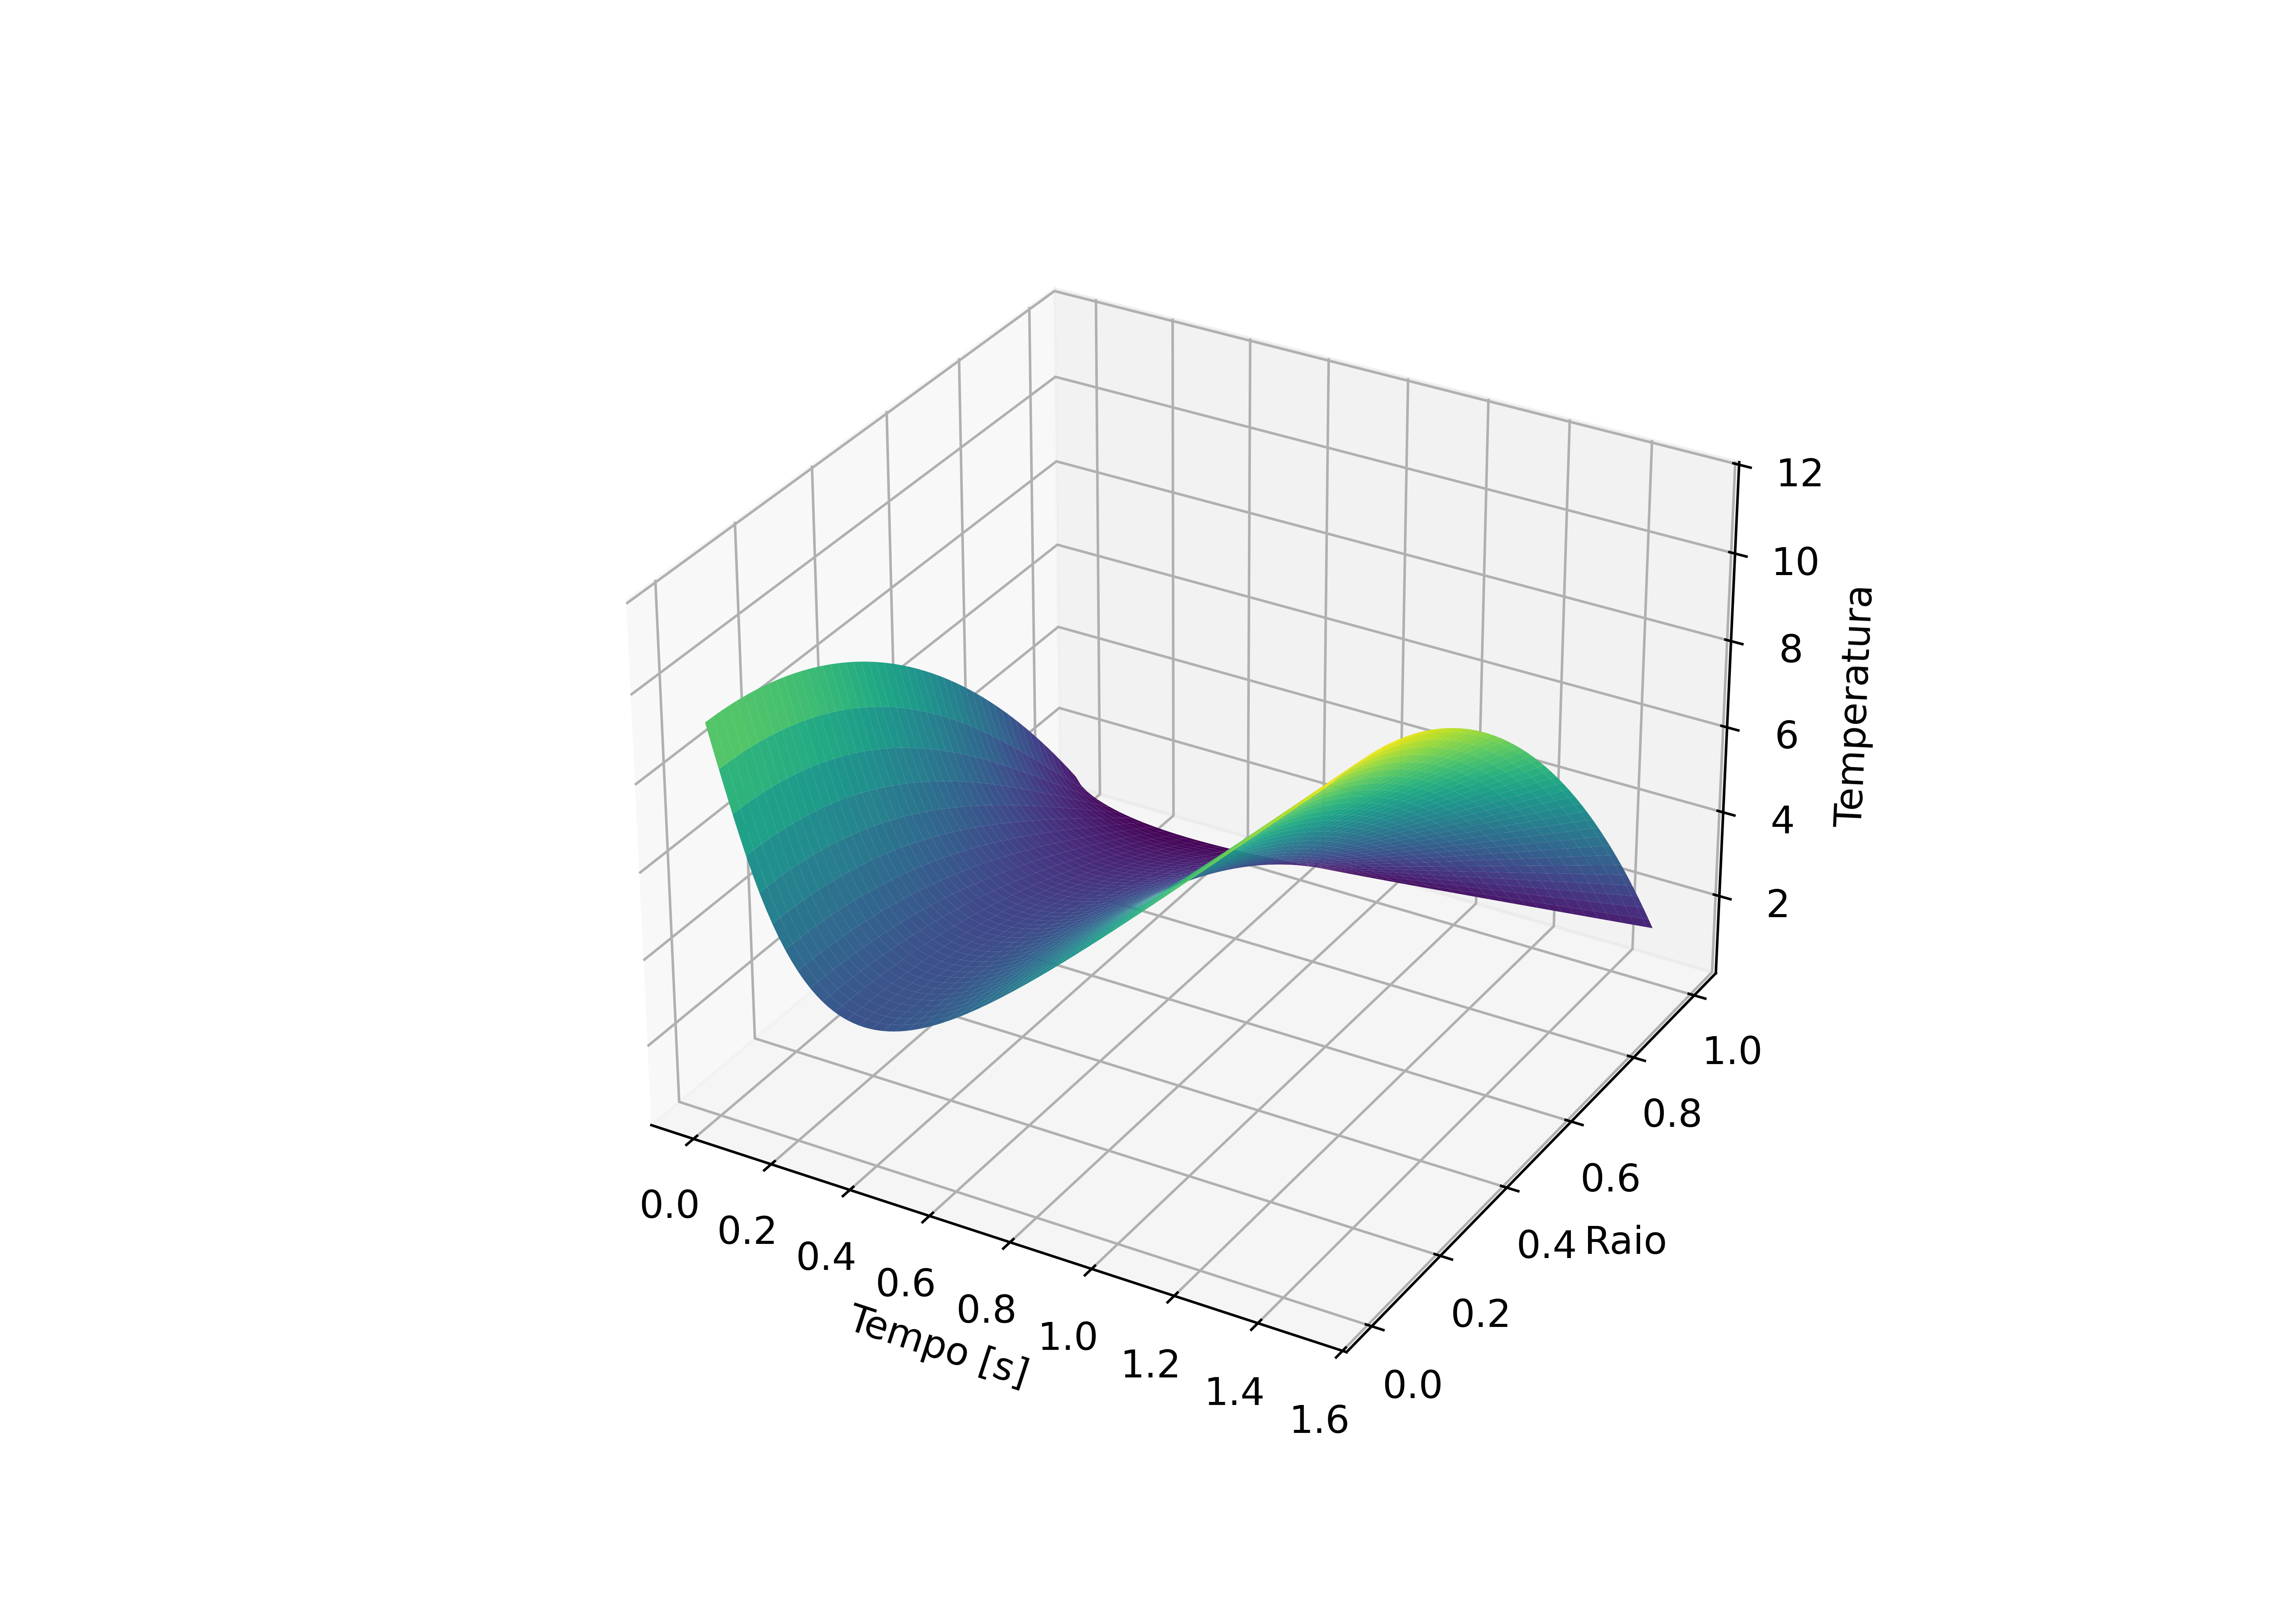
\includegraphics[width=1\linewidth]{figures/results/Fig01.png} 
        \caption{}
    \end{subfigure}
    \begin{subfigure}{0.45\textwidth}
        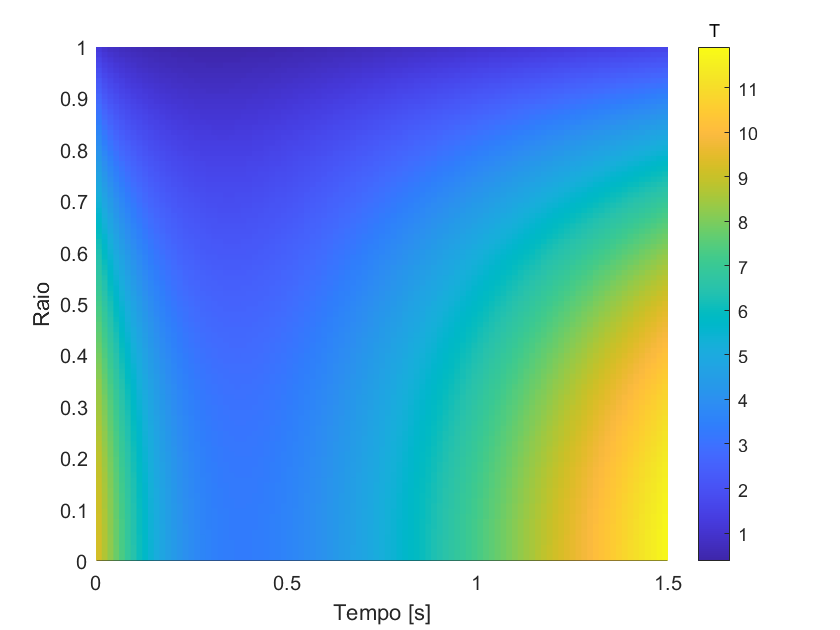
\includegraphics[width=1\linewidth]{figures/results/Fig02.png}
        \caption{}
    \end{subfigure}
    
    \source{Autor, 2023.}
    \label{fig:surface01}
\end{figure}

O perfil de temperatura apresentado na forma de superfície na Figura \ref{fig:surface01} apresenta o variação de temperatura (adimensionalizada) através do raio da vareta de combustível, considerando a primeira forma de geração de calor, conforme equação \ref{eq:first_form_of_heat}.

Ao longo de todo o período de tempo, a origem da vareta exibiu o valor máximo de temperatura, enquanto a extremidade manteve a temperatura mínima. Esse padrão era esperado, considerando a fonte de calor na origem, que se propaga ao longo da vareta em direção à extremidade e, por fim, a superfície da vareta apresentando um resfriamento convectivo.

Observou-se, ainda, que a origem da vareta demonstrou um comportamento com uma temperatura inicial elevada, passando por um processo de resfriamento, seguido de um subsequente aquecimento, algo que não era esperado.

\begin{figure}[H]
    \centering
    \caption{Comparativo de resultados com a literatura para primeira forma de geração de calor.}    
    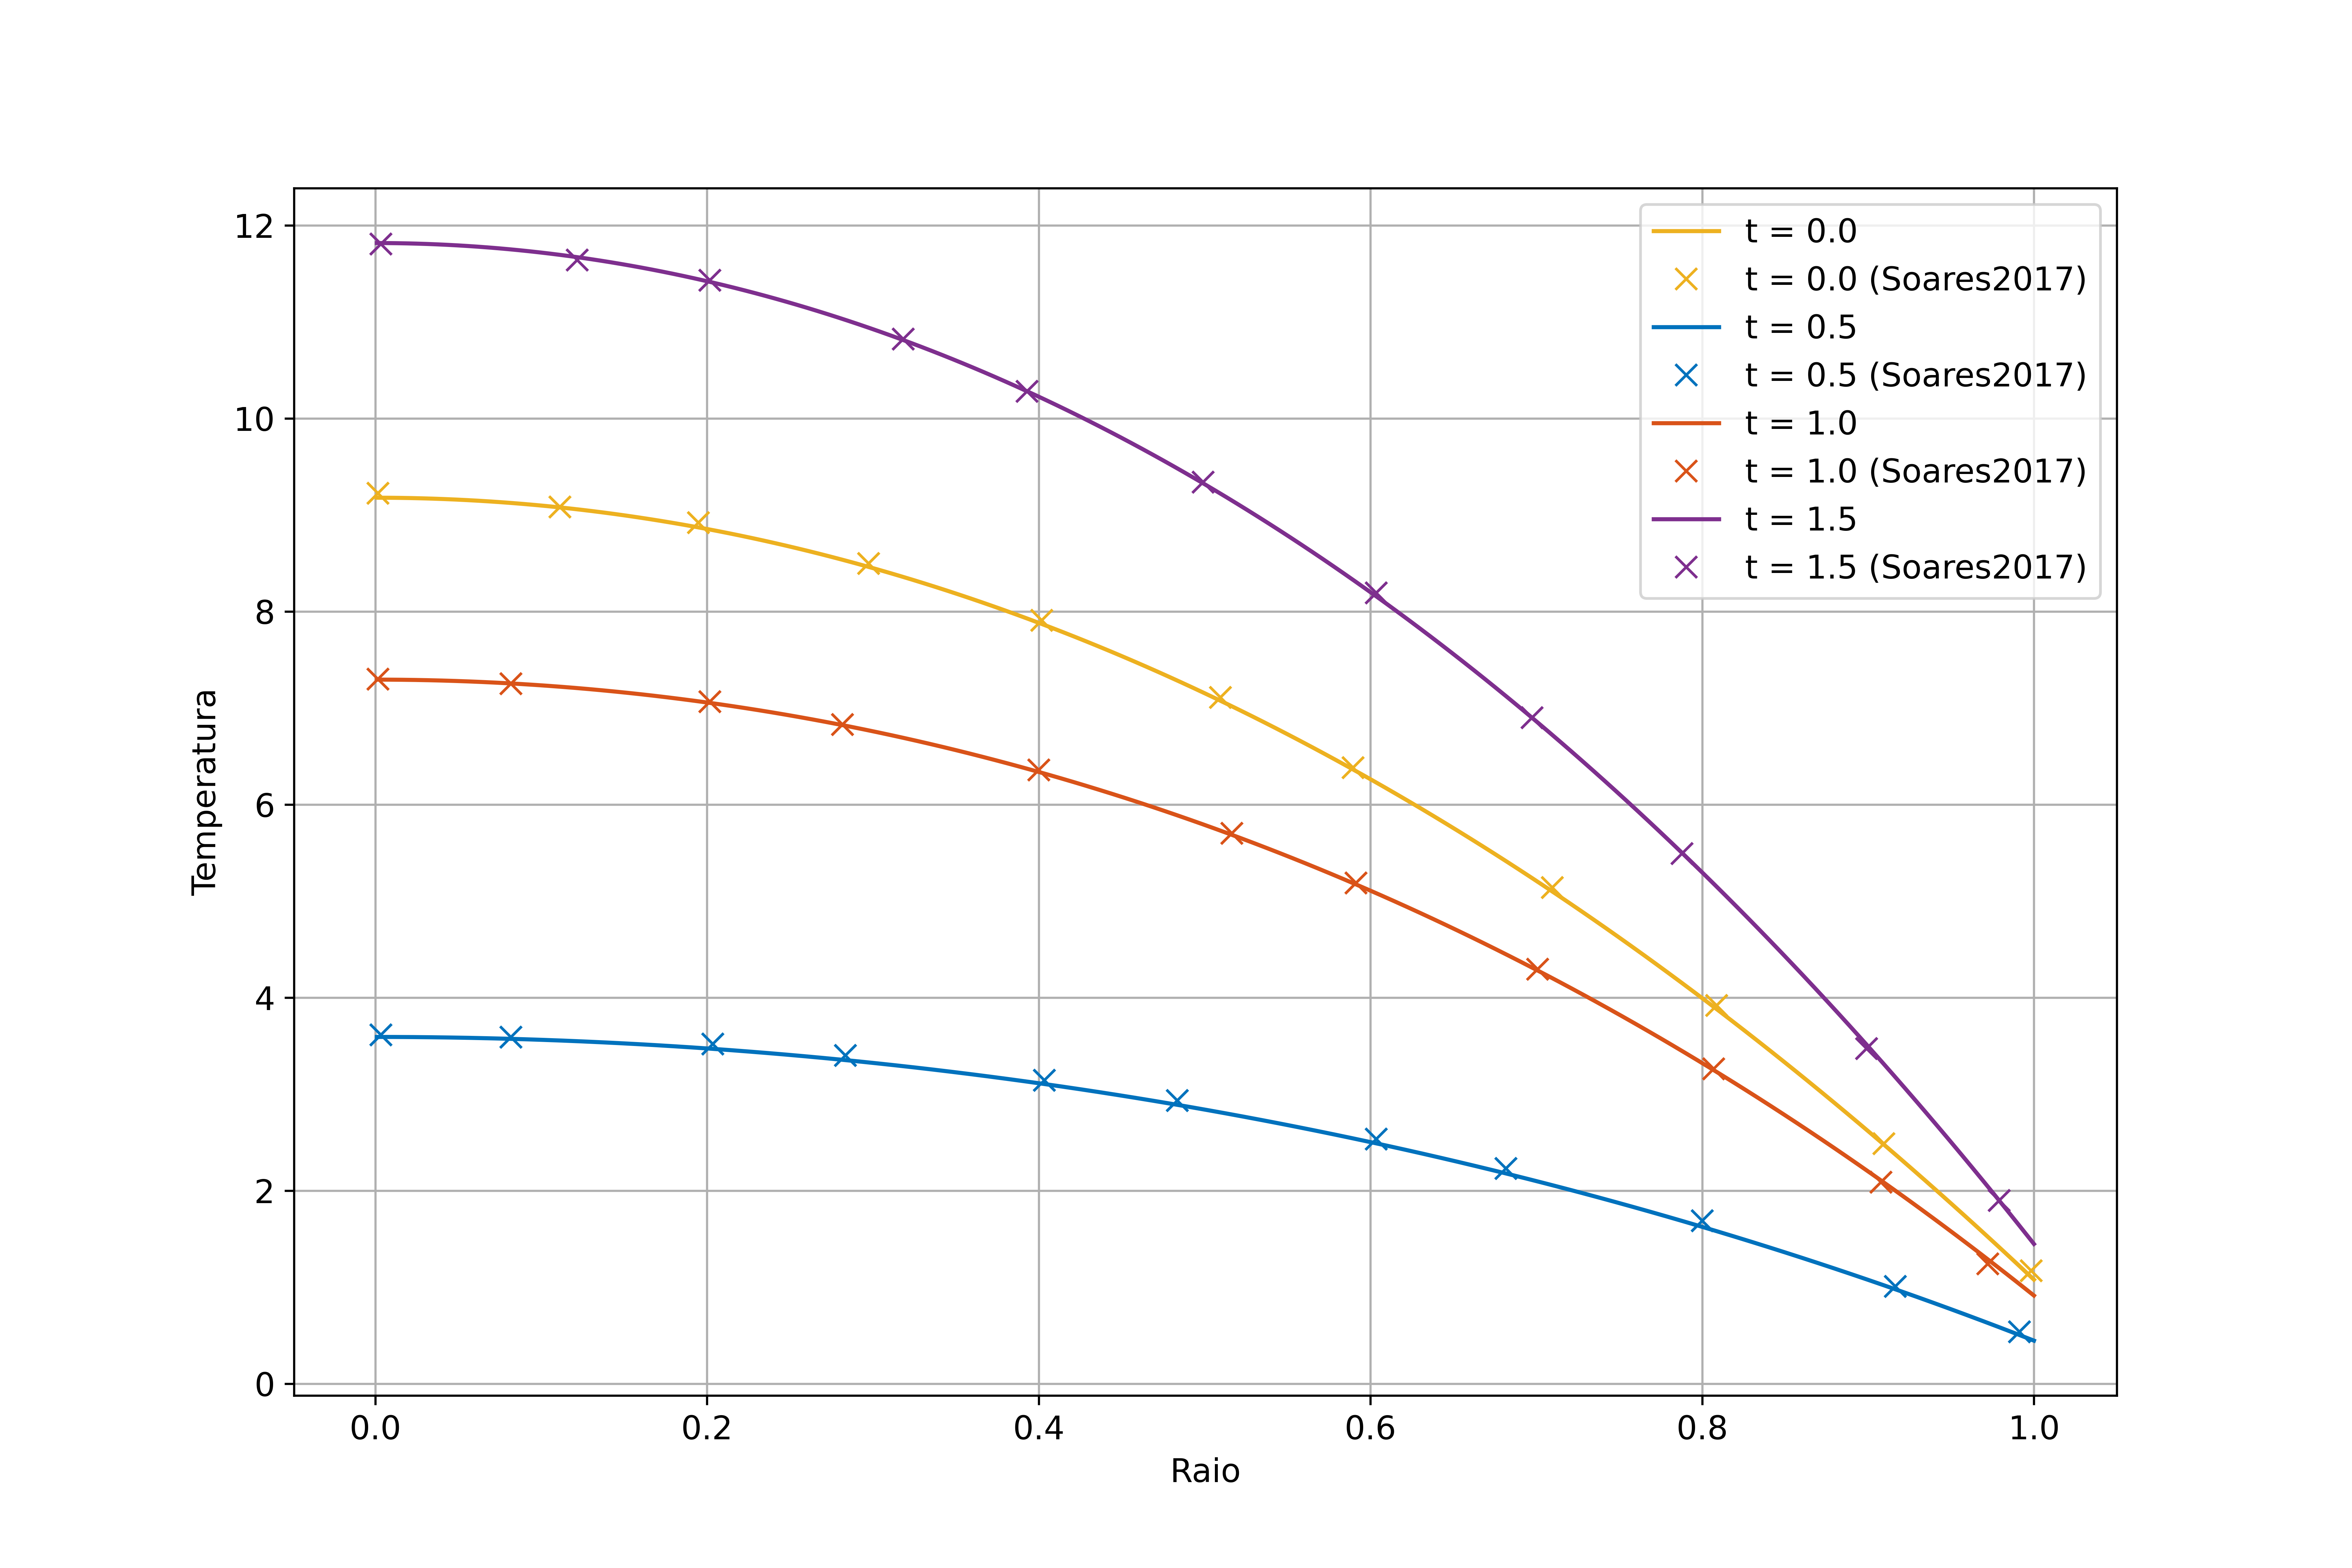
\includegraphics[scale=0.5]{figures/results/Fig03.png}
    \source{Autor, 2023.}
    \label{fig:profile01}
\end{figure}

Resultados análogos à Figura \ref{fig:surface01} foram apresentados na Figura \ref{fig:profile01}, mas dessa vez na forma de curvas para quatro instantes de tempos. Os resultados foram comparados com os apresentados por \citet{soares2017}, em todos os casos houve concordância entre os perfis de temperatura, com eventuais divergências decorrentes do método de obtenção dos dados, conforme supradito.

\subsection{Segunda Forma de Geração de Calor}

A segunda forma de geração de calor foi proposta por \citet{bhattacharya2001} e referenciada por \citet{soares2017}, ela se dá pela equação:

\begin{gather}
    G ' = G ^* r ^2 e ^{c_3 t}
    \label{eq:second_form_of_heat}
\end{gather}

\begin{figure}[H]
    \centering
    \caption{Perfis de temperatura para segunda forma de geração de calor: (a) perspectiva isométrica; (b) vista superior.}
    
    \begin{subfigure}{0.45\textwidth}
        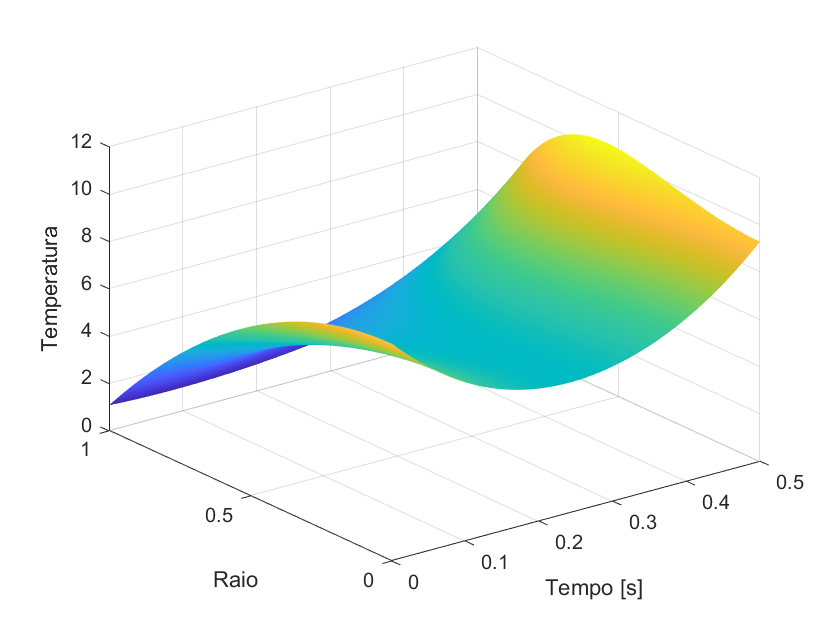
\includegraphics[width=1\linewidth]{figures/results/Fig04.png} 
        \caption{}
    \end{subfigure}
    \begin{subfigure}{0.45\textwidth}
        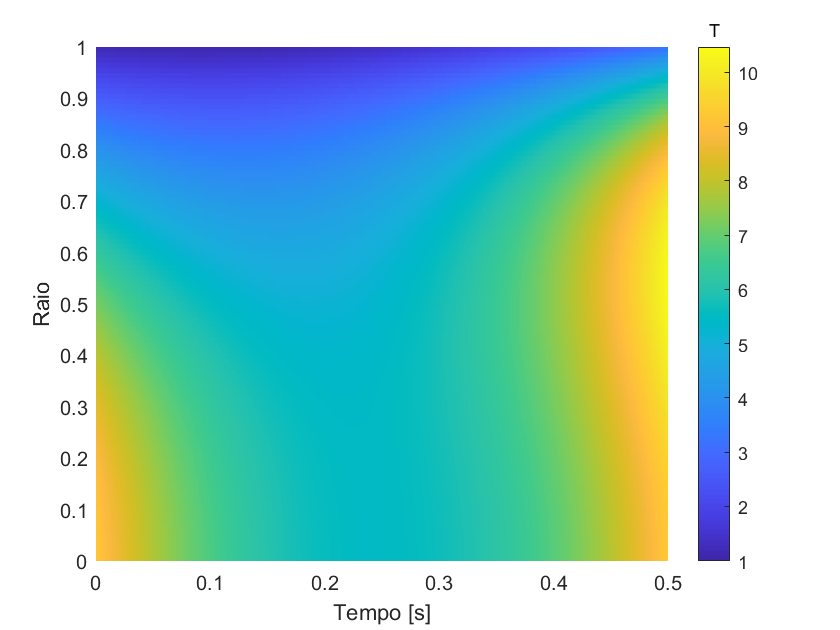
\includegraphics[width=1\linewidth]{figures/results/Fig05.png}
        \caption{}
    \end{subfigure}
    
    \source{Autor, 2023.}
    \label{fig:surface02}
\end{figure}

O perfil de temperatura apresentado na forma de superfície na Figura \ref{fig:surface02} apresenta o variação de temperatura (adimensionalizada) através do raio da vareta de combustível, considerando a segunda forma de geração de calor, conforme equação \ref{eq:second_form_of_heat}.

Para o presente caso, o intervalo de tempo foi reduzido para reproduzir o fenômeno de forma mais significativa.

Durante a maior parte do período de tempo a origem da vareta exibiu o valor máximo de temperatura, enquanto que a extremidade apresentou a temperatura mínima, porém com o passar do tempo (últimos instantes da simulação) houve uma transição do valor máximo da origem para a extremidade.

Observou-se, ainda, que que todos os pontos do raio demonstraram um comportamento de crescimento incessante de temperatura, com o passar do tempo, indicando que a geração de calor na origem superou o resfriamento na superfície.

\begin{figure}[H]
    \centering
    \caption{Comparativo de resultados com a literatura para segunda forma de geração de calor.}
    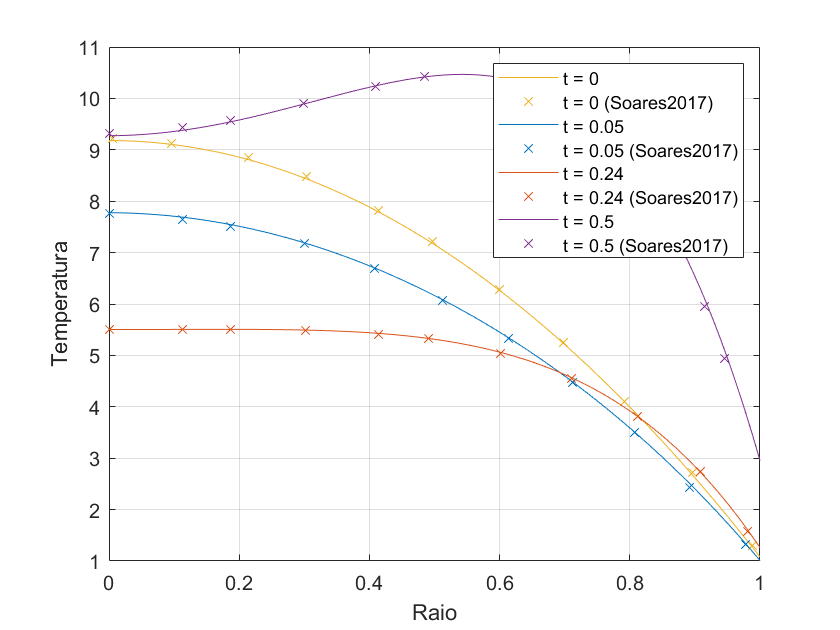
\includegraphics[scale=0.5]{figures/results/Fig06.png}
    \source{Autor, 2023.}
    \label{fig:profile02}
\end{figure}

Resultados análogos à Figura \ref{fig:surface02} foram apresentados na Figura \ref{fig:profile02}, mas dessa vez na forma de curvas para quatro instantes de tempos. Os resultados foram comparados com os apresentados por \citet{soares2017}, em todos os casos houve concordância entre os perfis de temperatura, com eventuais divergências decorrentes do método de obtenção dos dados, conforme supradito.

\subsection{Terceira Forma de Geração de Calor}

A terceira forma de geração de calor foi proposta por \citet{soares2017}, ela se dá pela equação:

\begin{gather}
    G ' = G ^* (1 + c _1 t)
    \label{eq:third_form_of_heat}
\end{gather}

Nela, o valor do coeficiente \(c_1\) foi considerado igual a \(1\), seguindo a literatura.

\begin{figure}[H]
    \centering
    \caption{Perfis de temperatura para terceira forma de geração de calor: (a) perspectiva isométrica; (b) vista superior.}
    
    \begin{subfigure}{0.45\textwidth}
        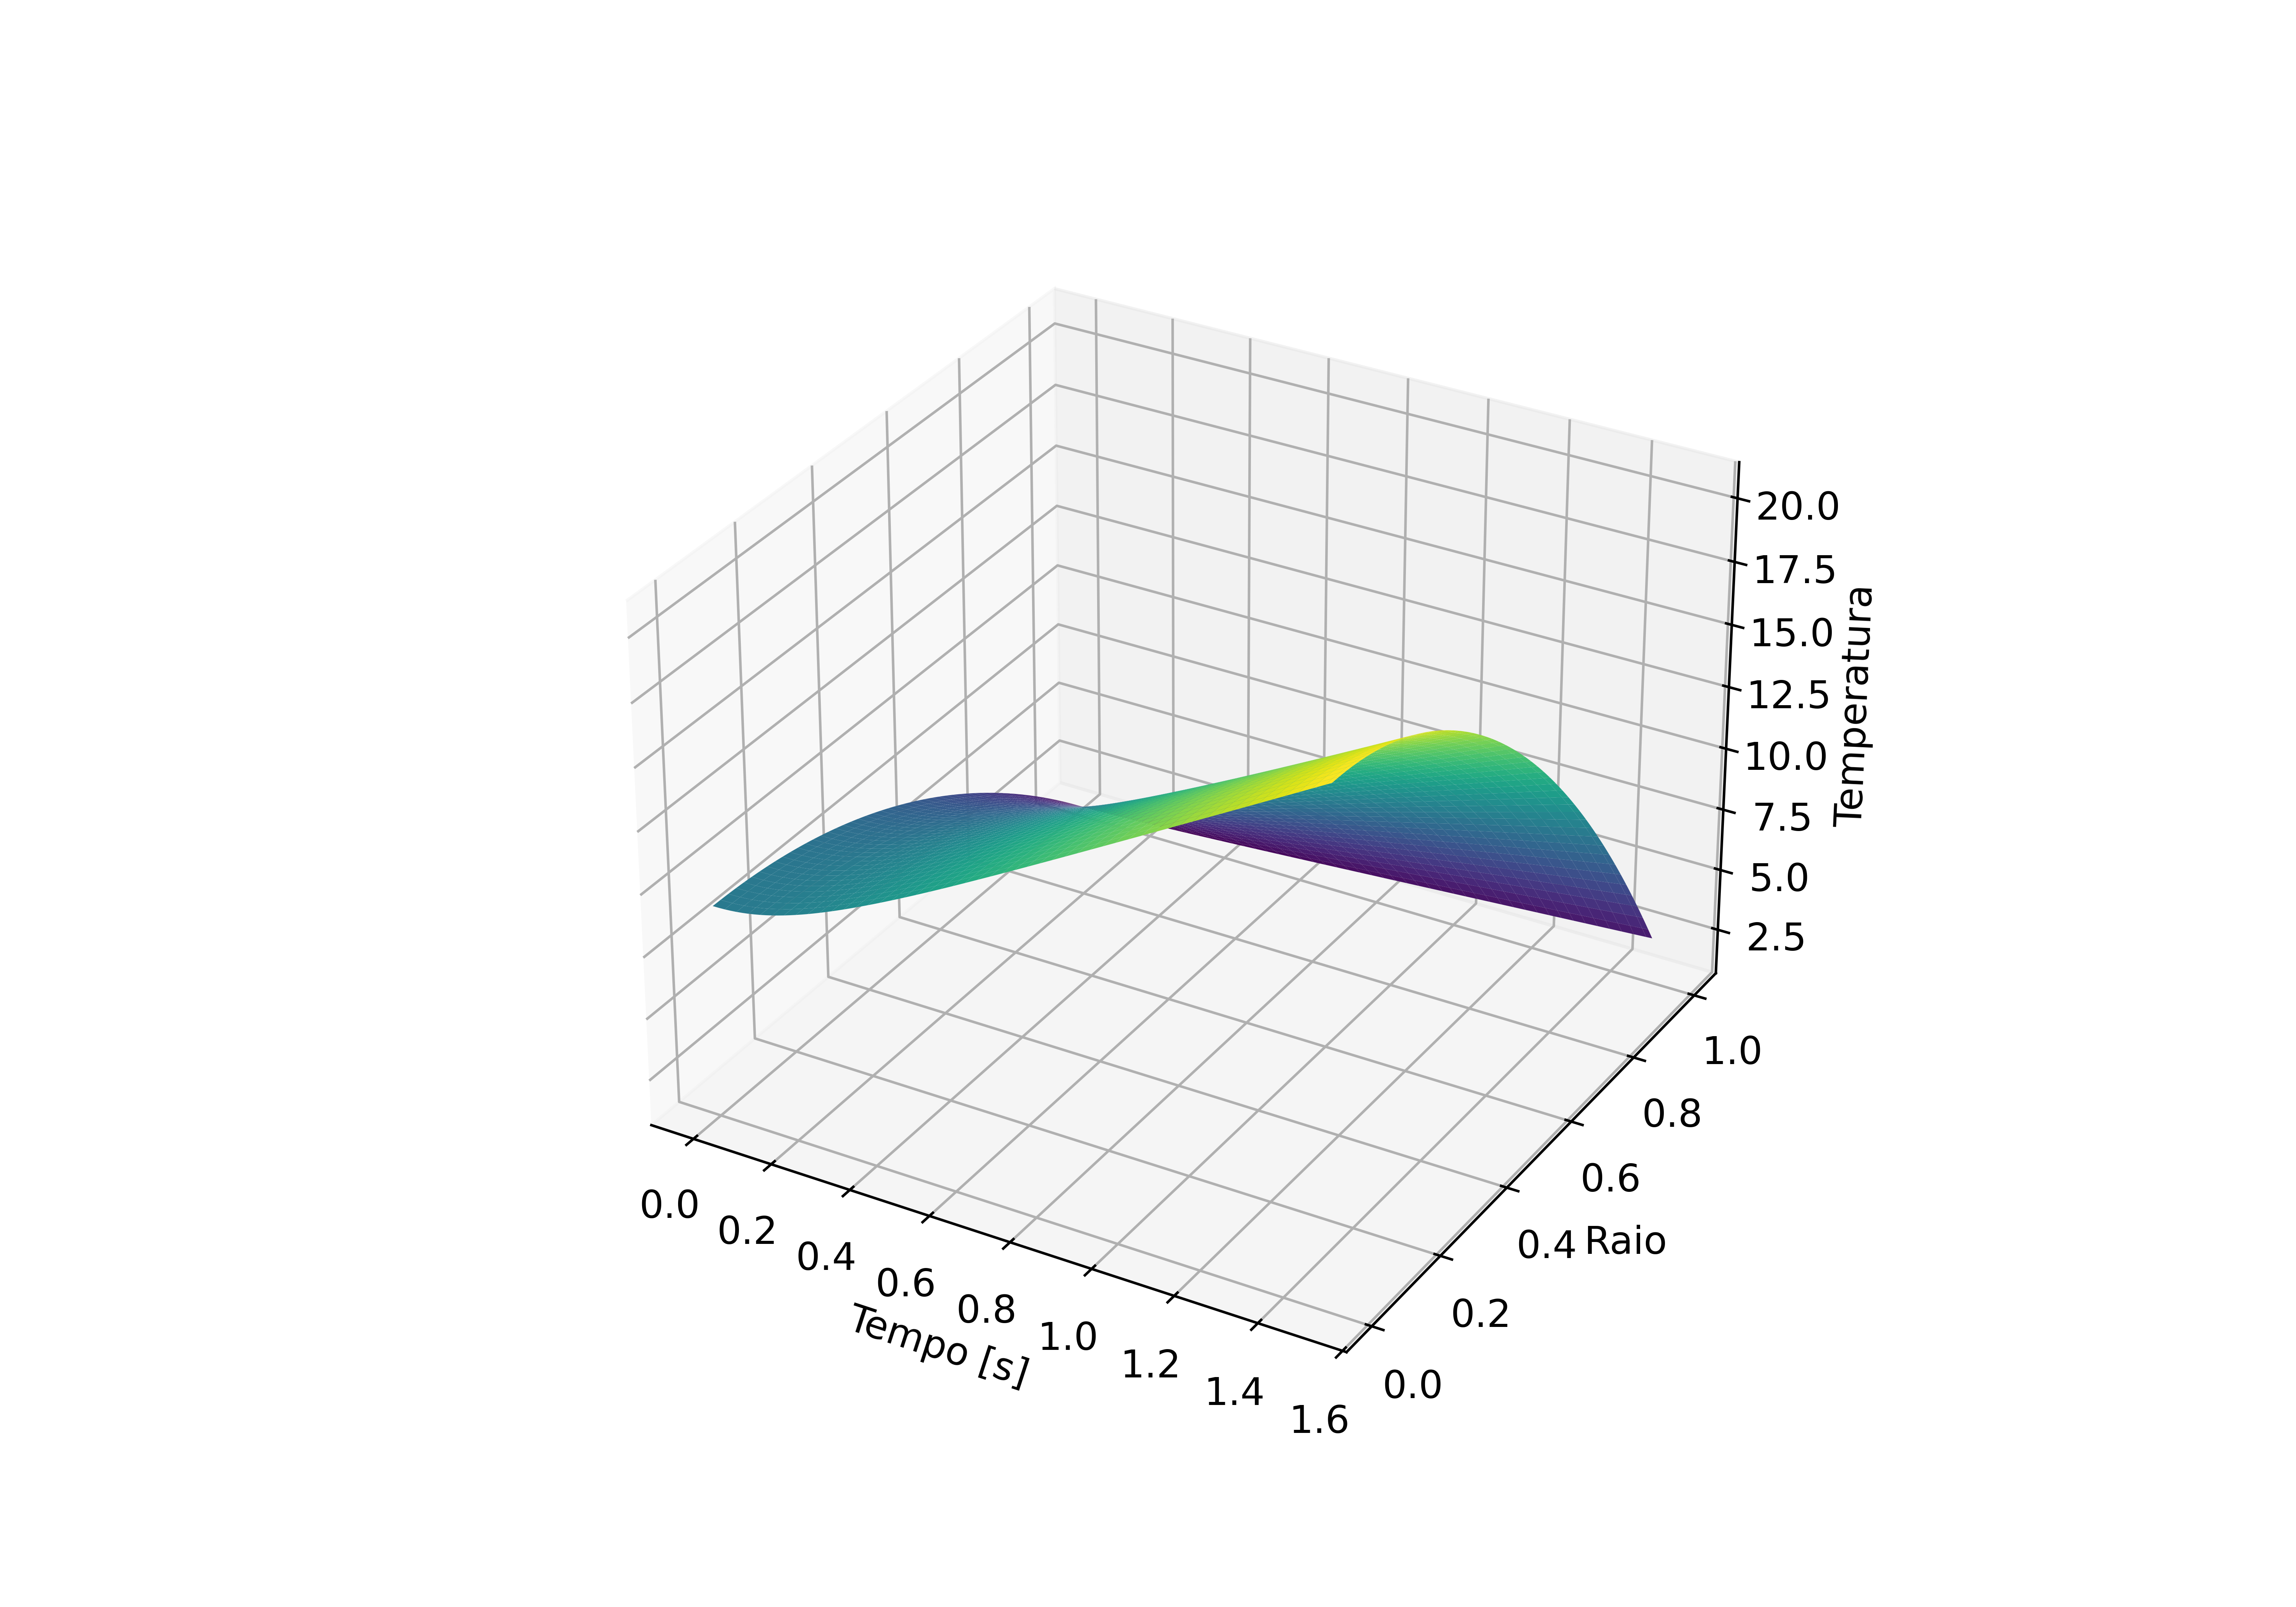
\includegraphics[width=1\linewidth]{figures/results/Fig07.png} 
        \caption{}
    \end{subfigure}
    \begin{subfigure}{0.45\textwidth}
        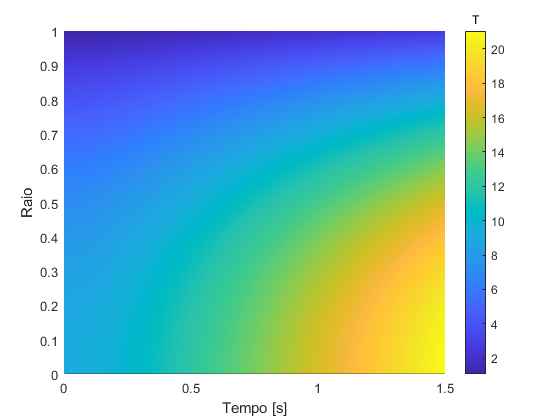
\includegraphics[width=1\linewidth]{figures/results/Fig08.png}
        \caption{}
    \end{subfigure}
    
    \source{Autor, 2023.}
    \label{fig:surface03}
\end{figure}

O perfil de temperatura apresentado na forma de superfície na Figura \ref{fig:surface03} apresenta o variação de temperatura (adimensionalizada) através do raio da vareta de combustível, considerando a terceira forma de geração de calor, conforme equação \ref{eq:third_form_of_heat}.

De forma análoga a primeira forma de geração de calor, ao longo de todo o período de tempo, a origem da vareta exibiu o valor máximo de temperatura, enquanto a extremidade manteve a temperatura mínima. Novamente, esse padrão era esperado, considerando a fonte de calor na origem, que se propaga ao longo da vareta em direção à extremidade e, por fim, a superfície da vareta apresentando um resfriamento convectivo.

Observou-se, ainda, que com o passar do tempo houve um aumento expressivo de temperatura na origem com propagação para a região da superfície, indicando que com o passar do tempo a geração de calor tendeu a superar o resfriamento na superfície.

\begin{figure}[H]
    \centering
    \caption{Comparativo de resultados com a literatura para terceira forma de geração de calor.}
    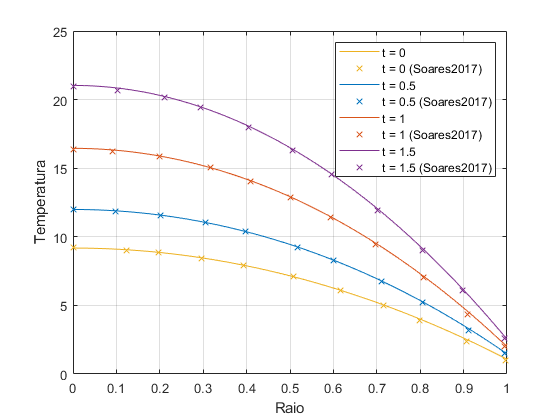
\includegraphics[scale=0.7]{figures/results/Fig09.png}
    \source{Autor, 2023.}
    \label{fig:profile03}
\end{figure}

Resultados análogos à Figura \ref{fig:surface03} foram apresentados na Figura \ref{fig:profile03}, mas dessa vez na forma de curvas para quatro instantes de tempos. Os resultados foram comparados com os apresentados por \citet{soares2017}, em todos os casos houve concordância entre os perfis de temperatura, com eventuais divergências decorrentes do método de obtenção dos dados, conforme supradito.

\begin{figure}[H]
    \centering
    \caption{Influência nos perfis de temperatura devido a variação no coeficiente \(c_1\) da terceira forma de geração de calor.}
    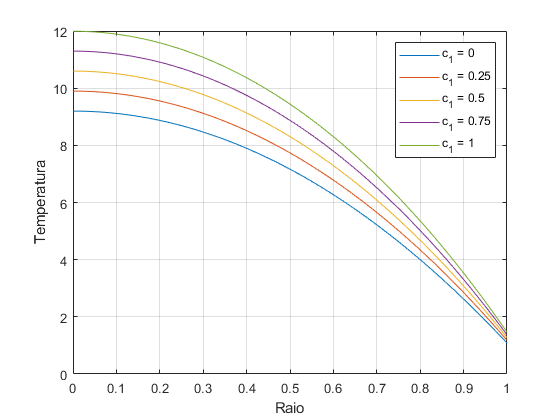
\includegraphics[scale=0.7]{figures/results/Fig10.png}
    \source{Autor, 2023.}
    \label{fig:influence_of_coefficient_c1}
\end{figure}

Em seguida, buscou-se estudar a influência do coeficiente \(c_1\) nos perfis de temperatura. Através da Figura \ref{fig:influence_of_coefficient_c1} pode-se observar que com o aumento do valor do coeficiente, houve um aumento dos valores de temperatura, algo esperado devido a expressão da geração de calor.

\begin{figure}[H]
    \centering
    \caption{Influência nos perfis de temperatura devido a variação no número de \(Bi\) na terceira forma de geração de calor.}
    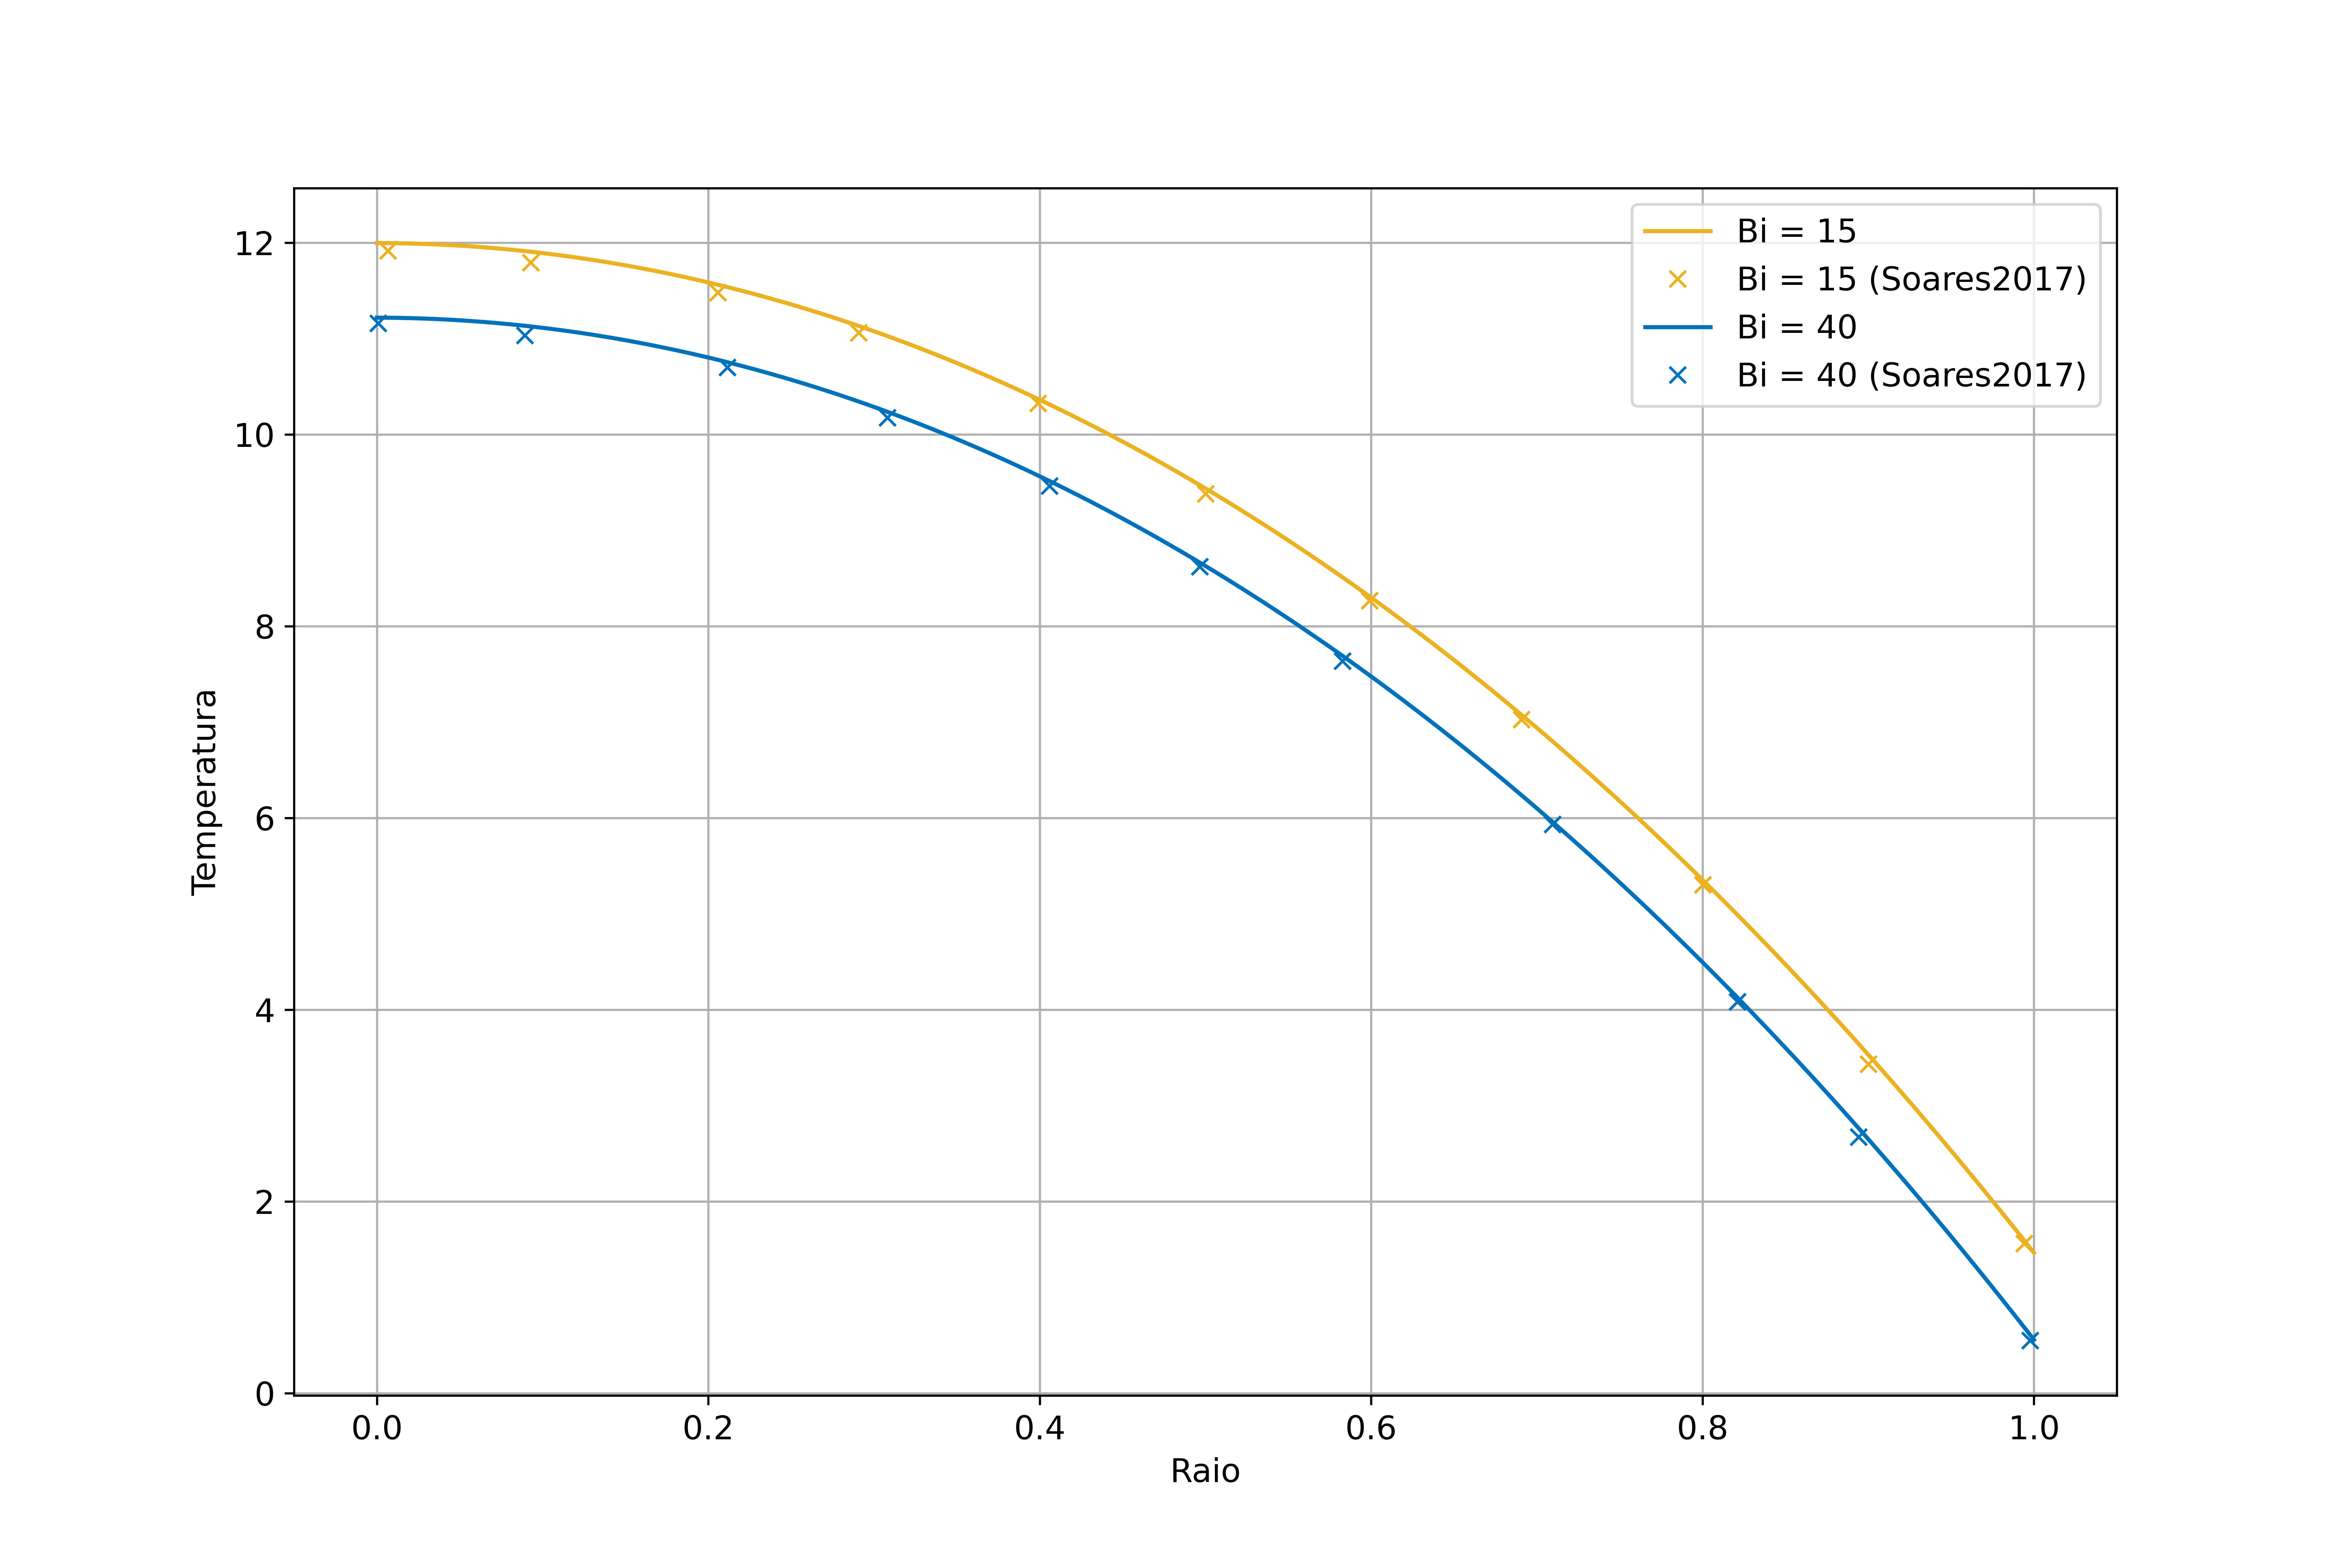
\includegraphics[scale=0.7]{figures/results/Fig11.png}
    \source{Autor, 2023.}
    \label{fig:influence_of_Biot_on_third_heat_generation}
\end{figure}

Por fim, buscou-se estudar a influência do número de Biot nos perfis de temperatura. Através da Figura \ref{fig:influence_of_Biot_on_third_heat_generation} pode-se observar que com o aumento do número de Biot, houve um descréscimo dos valores de temperatura, algo esperado devido a interpretação do mesmo (razão entre o coeficiente de transferência convectiva de calor na superfície e a condutância específica).

\subsection{Quarta Forma de Geração de Calor}

A quarta forma de geração de calor foi proposta por \citet{soares2017}, ela se dá pela equação:

\begin{gather}
    G ' = G ^* (1 + c_2 r ^2) e ^{c_3 t}
    \label{eq:fourth_form_of_heat}
\end{gather}

Nela, os coeficientes \(c_2\) e \(c_3\) foram considerados ambos iguais a \(1\), seguindo a literatura.

\begin{figure}[H]
    \centering
    \caption{Perfis de temperatura para quarta forma de geração de calor: (a) perspectiva isométrica; (b) vista superior.}
    
    \begin{subfigure}{0.45\textwidth}
        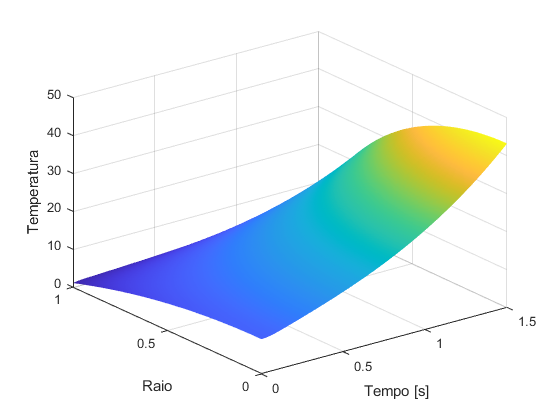
\includegraphics[width=1\linewidth]{figures/results/Fig12.png} 
        \caption{}
    \end{subfigure}
    \begin{subfigure}{0.45\textwidth}
        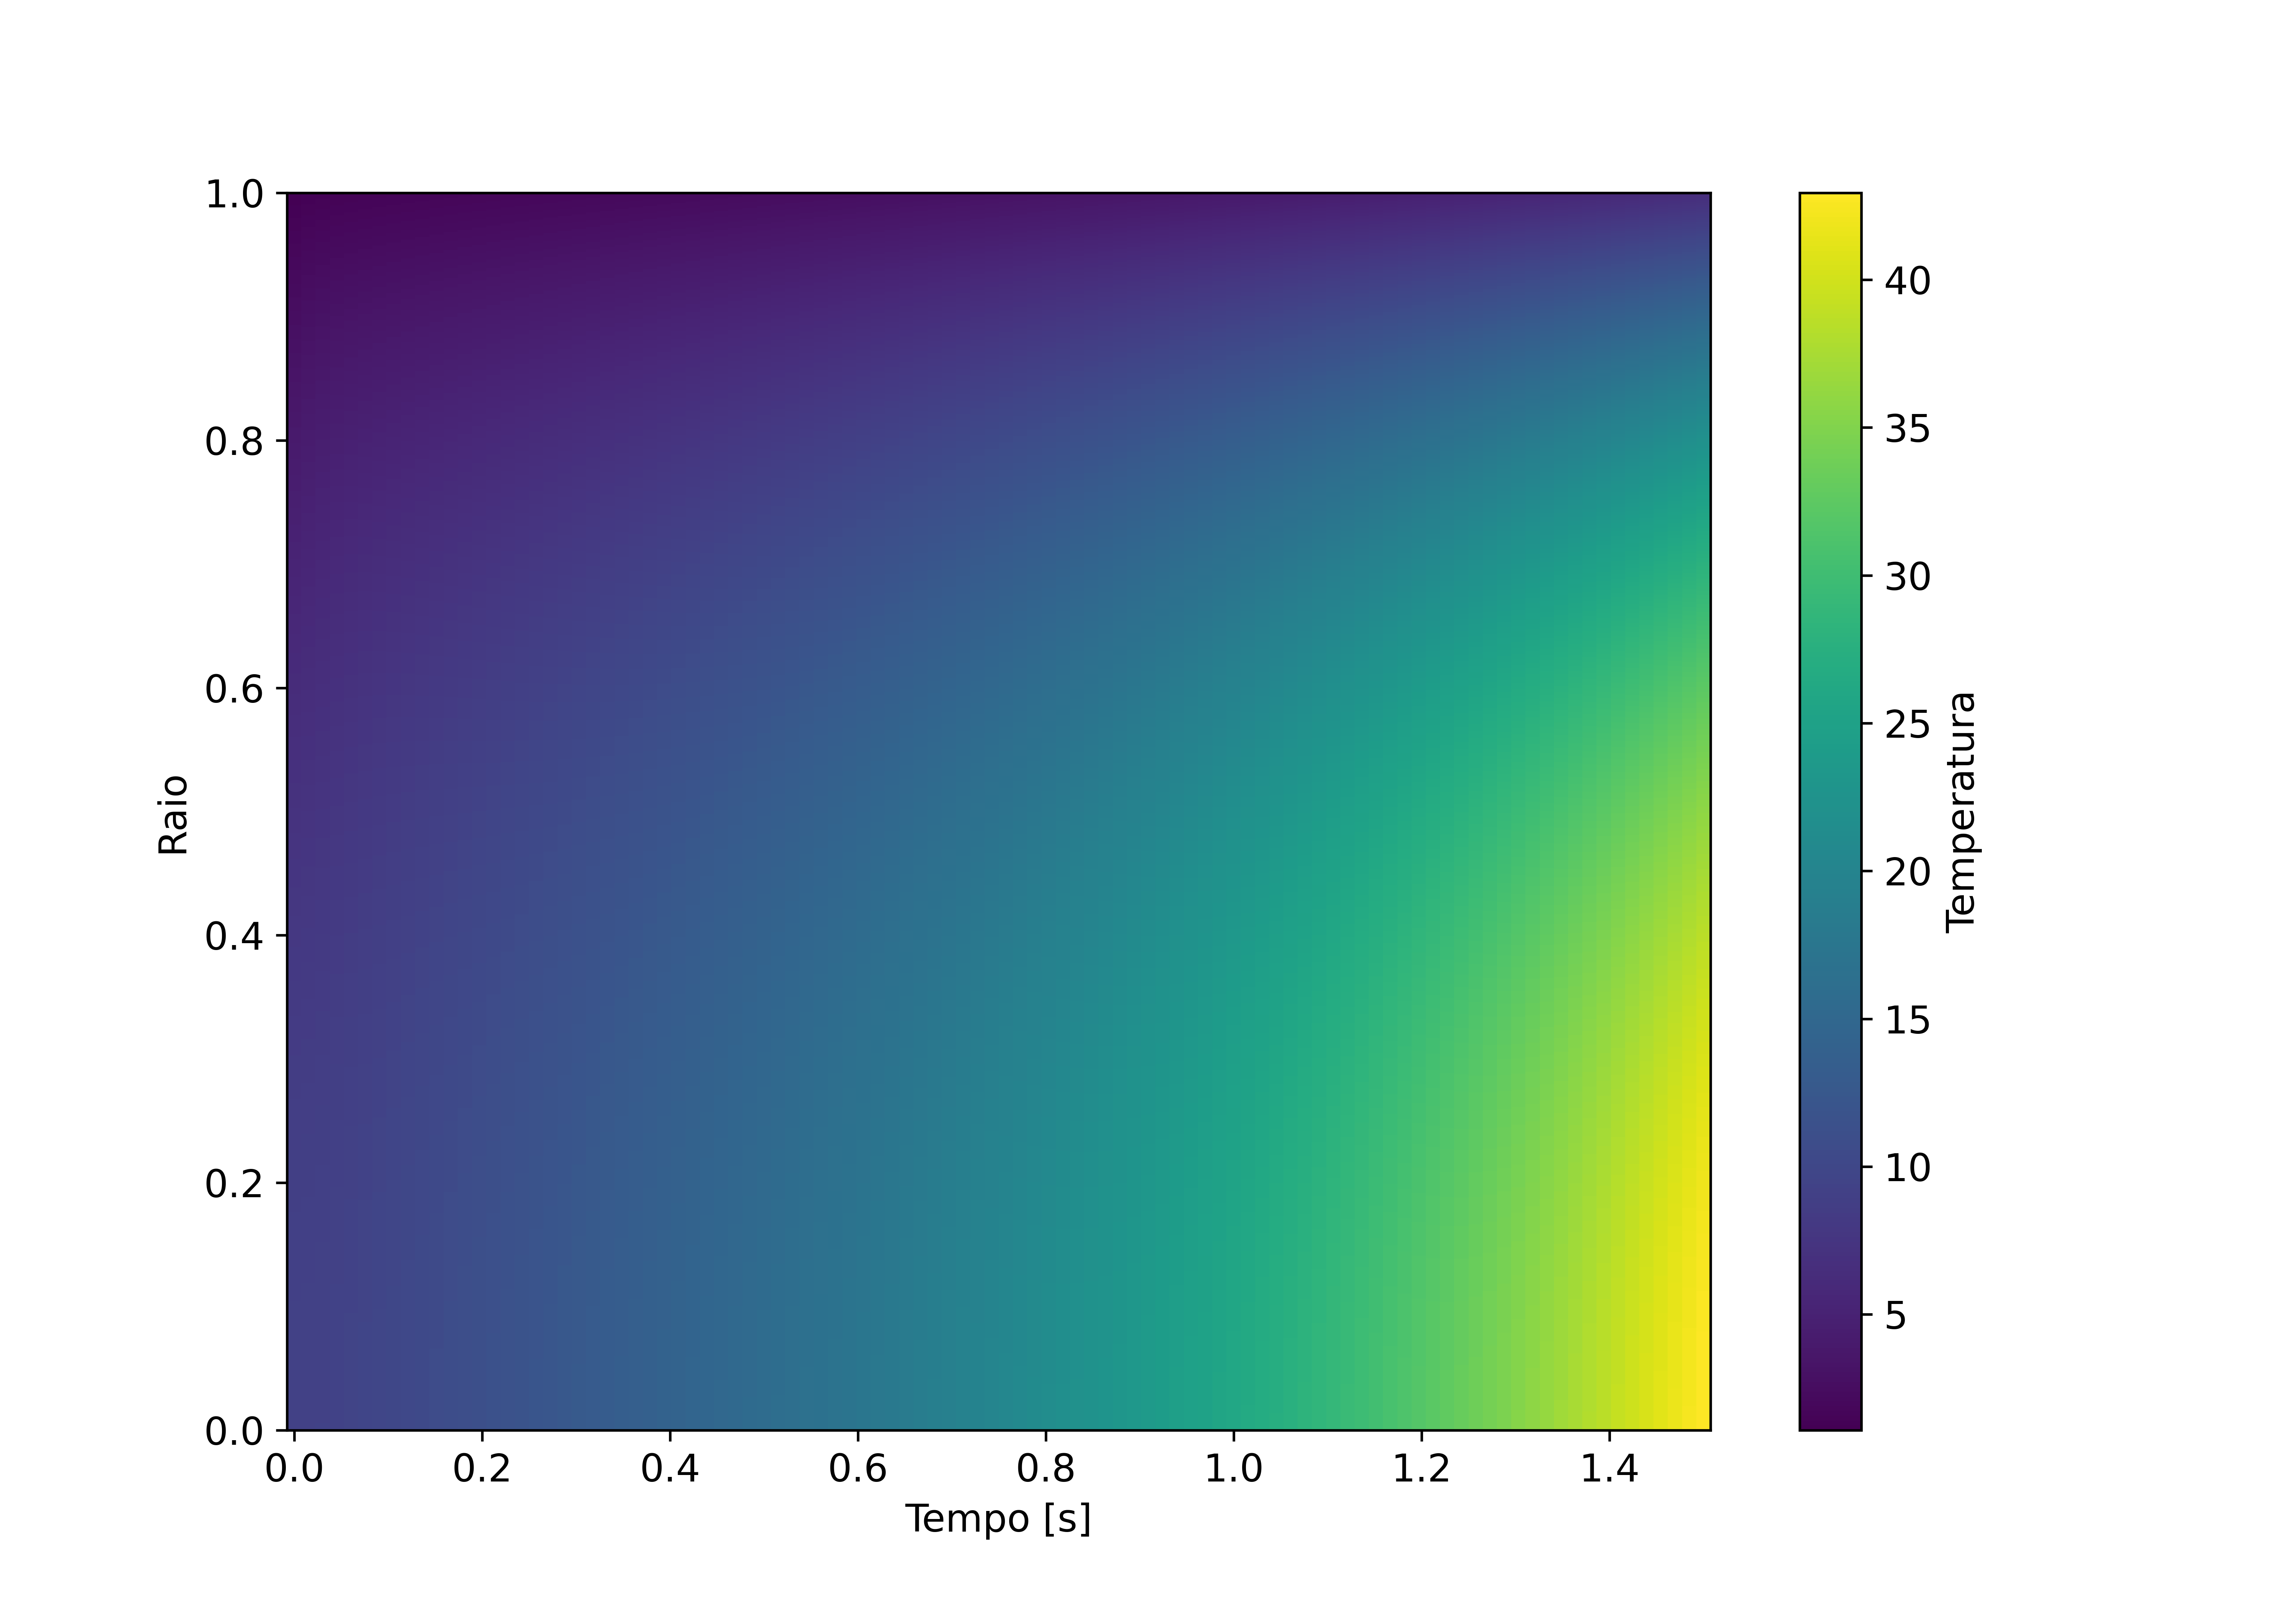
\includegraphics[width=1\linewidth]{figures/results/Fig13.png}
        \caption{}
    \end{subfigure}
    
    \source{Autor, 2023.}
    \label{fig:surface04}
\end{figure}

O perfil de temperatura apresentado na forma de superfície na Figura \ref{fig:surface04} apresenta o variação de temperatura (adimensionalizada) através do raio da vareta de combustível, considerando a quarta forma de geração de calor, conforme equação \ref{eq:fourth_form_of_heat}.

De forma análoga a terceira forma de geração de calor, ao longo de todo o período de tempo, a origem da vareta exibiu o valor máximo de temperatura, enquanto a extremidade manteve a temperatura mínima. Novamente, esse padrão era esperado, considerando a fonte de calor na origem, que se propaga ao longo da vareta em direção à extremidade e, por fim, a superfície da vareta apresentando um resfriamento convectivo.

Observou-se, ainda, que com o passar do tempo houve um aumento expressivo de temperatura na origem com propagação para a região da superfície, indicando que com o passar do tempo a geração de calor tendeu a superar o resfriamento na superfície.

\begin{figure}[H]
    \centering
    \caption{Comparativo de resultados com a literatura para quarta forma de geração de calor.}
    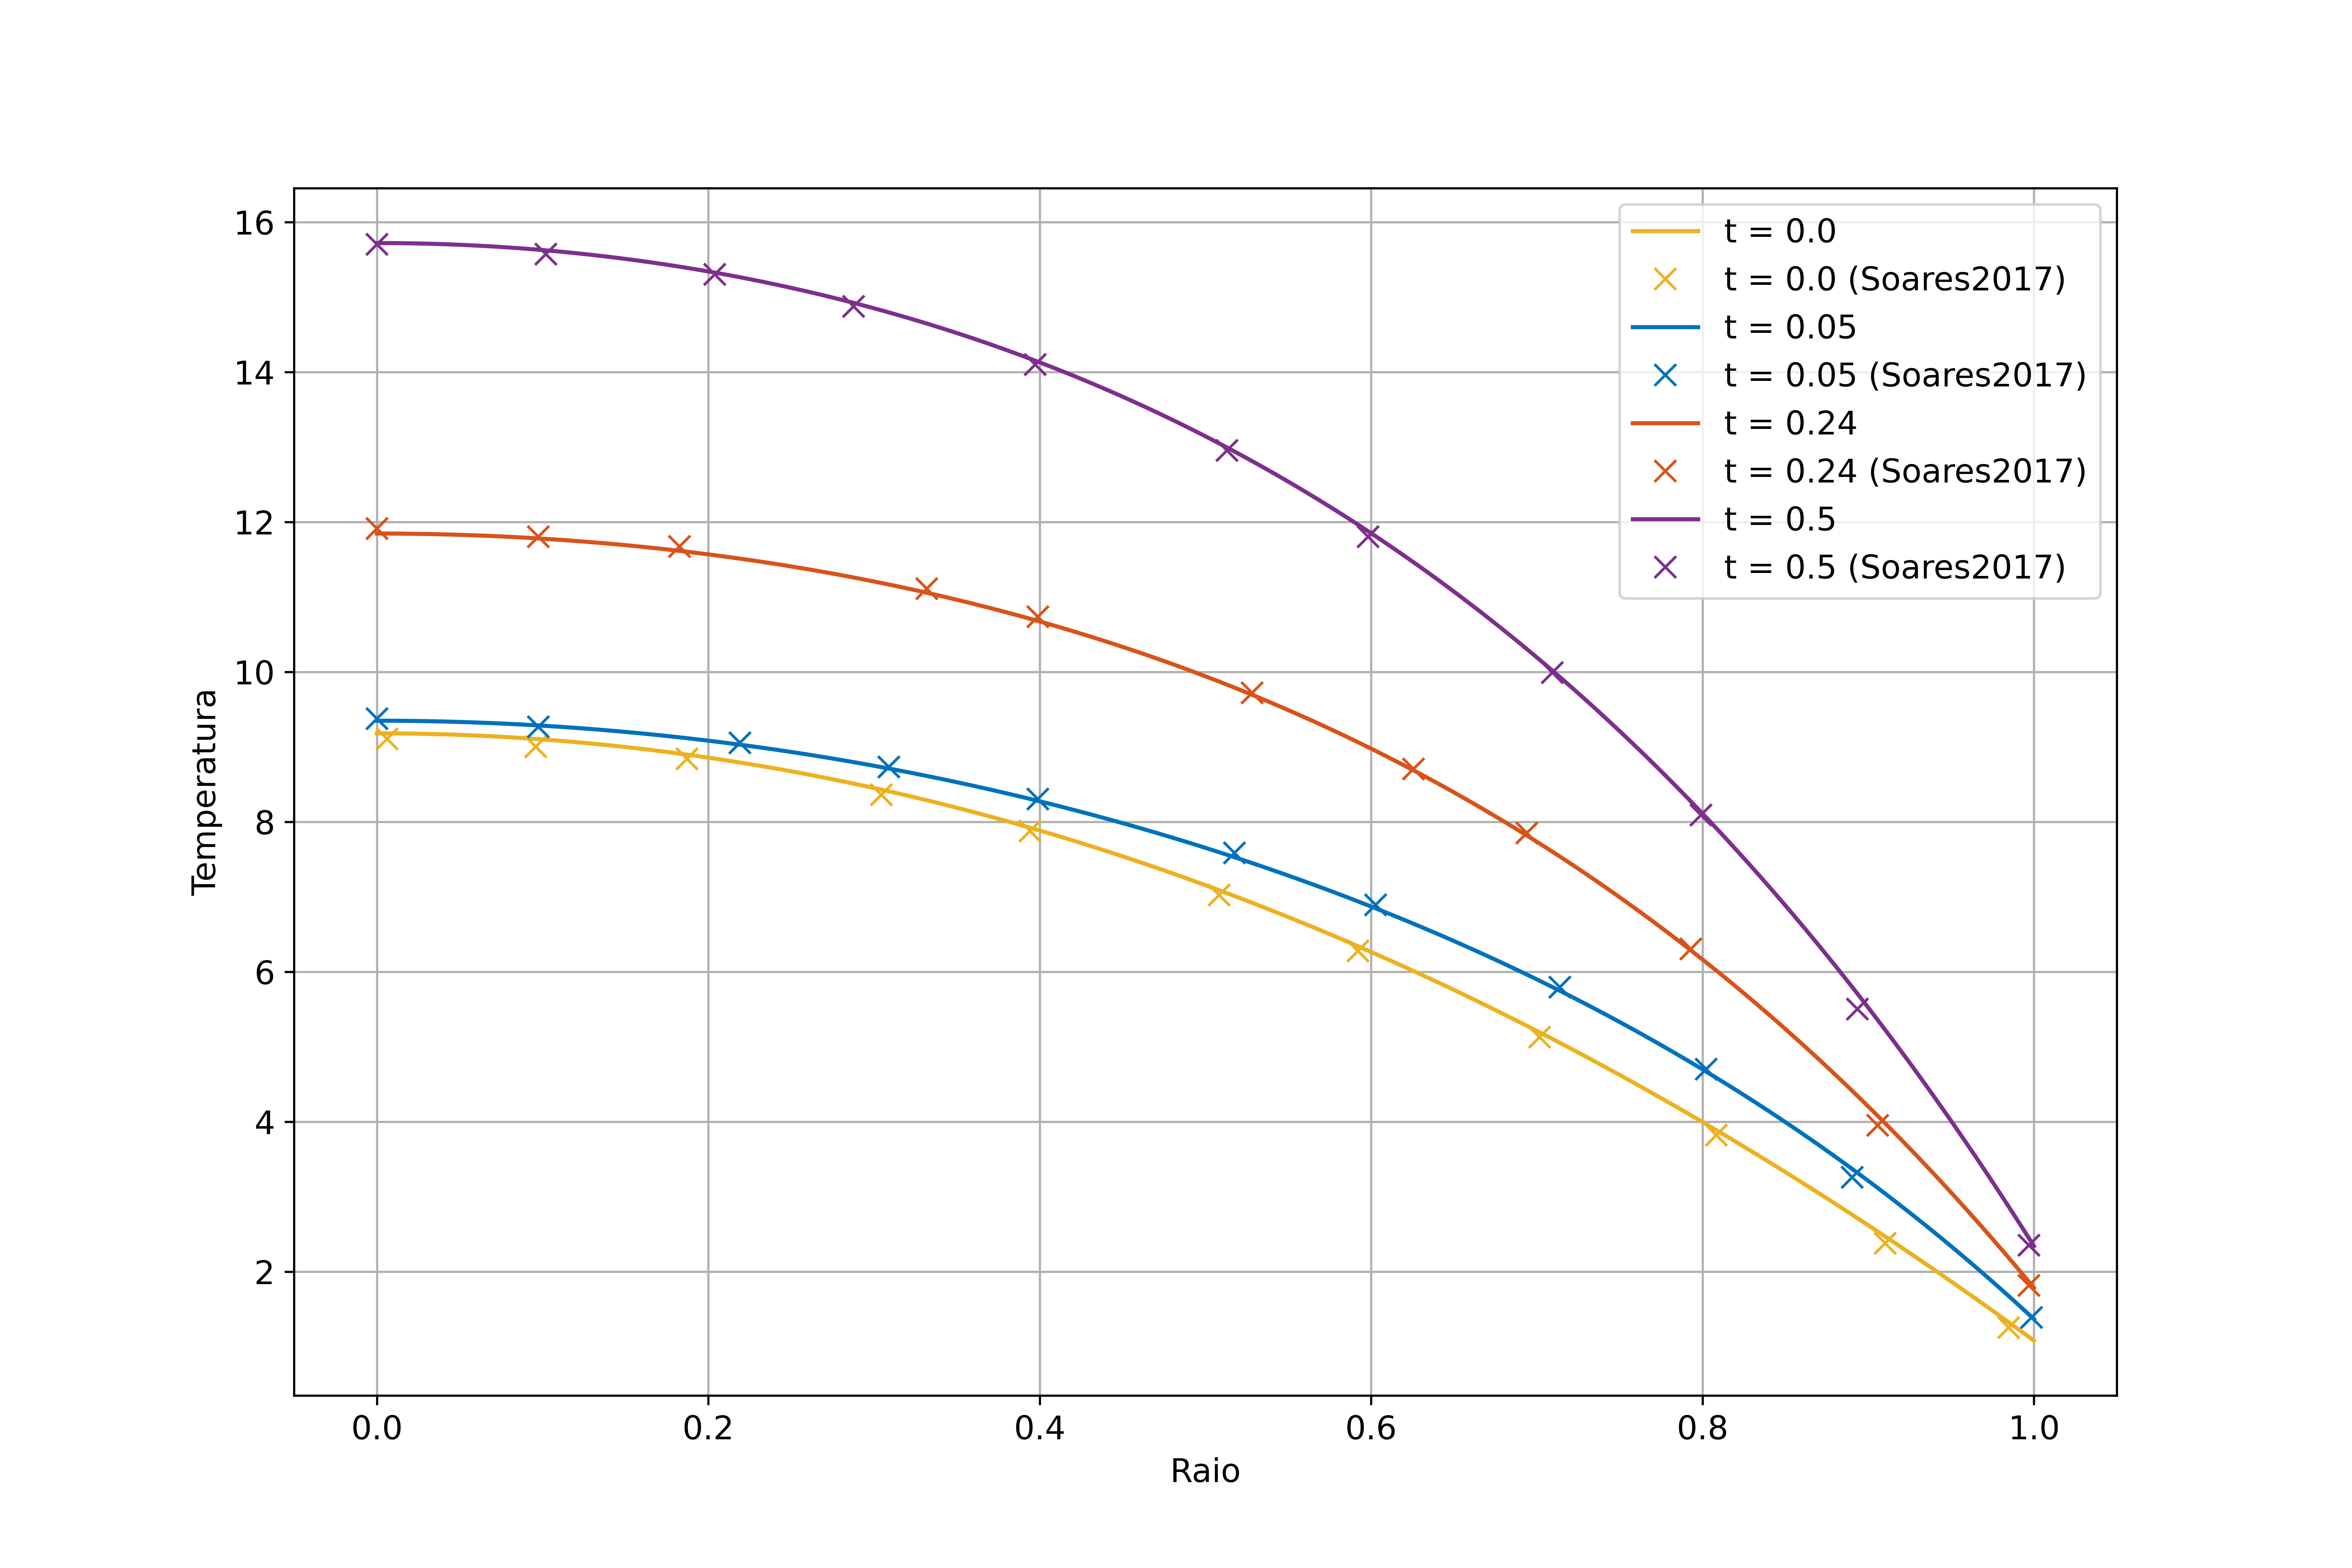
\includegraphics[scale=0.7]{figures/results/Fig14.png}
    \source{Autor, 2023.}
    \label{fig:profile04}
\end{figure}

Resultados análogos à Figura \ref{fig:surface04} foram apresentados na Figura \ref{fig:profile04}, mas dessa vez na forma de curvas para quatro instantes de tempos. Os resultados foram comparados com os apresentados por \citet{soares2017}, em todos os casos houve concordância entre os perfis de temperatura, com eventuais divergências decorrentes do método de obtenção dos dados, conforme supradito.

\begin{figure}[H]
    \centering
    \caption{Influência nos perfis de temperatura devido a variação no número de \(Bi\) na quarta forma de geração de calor.}
    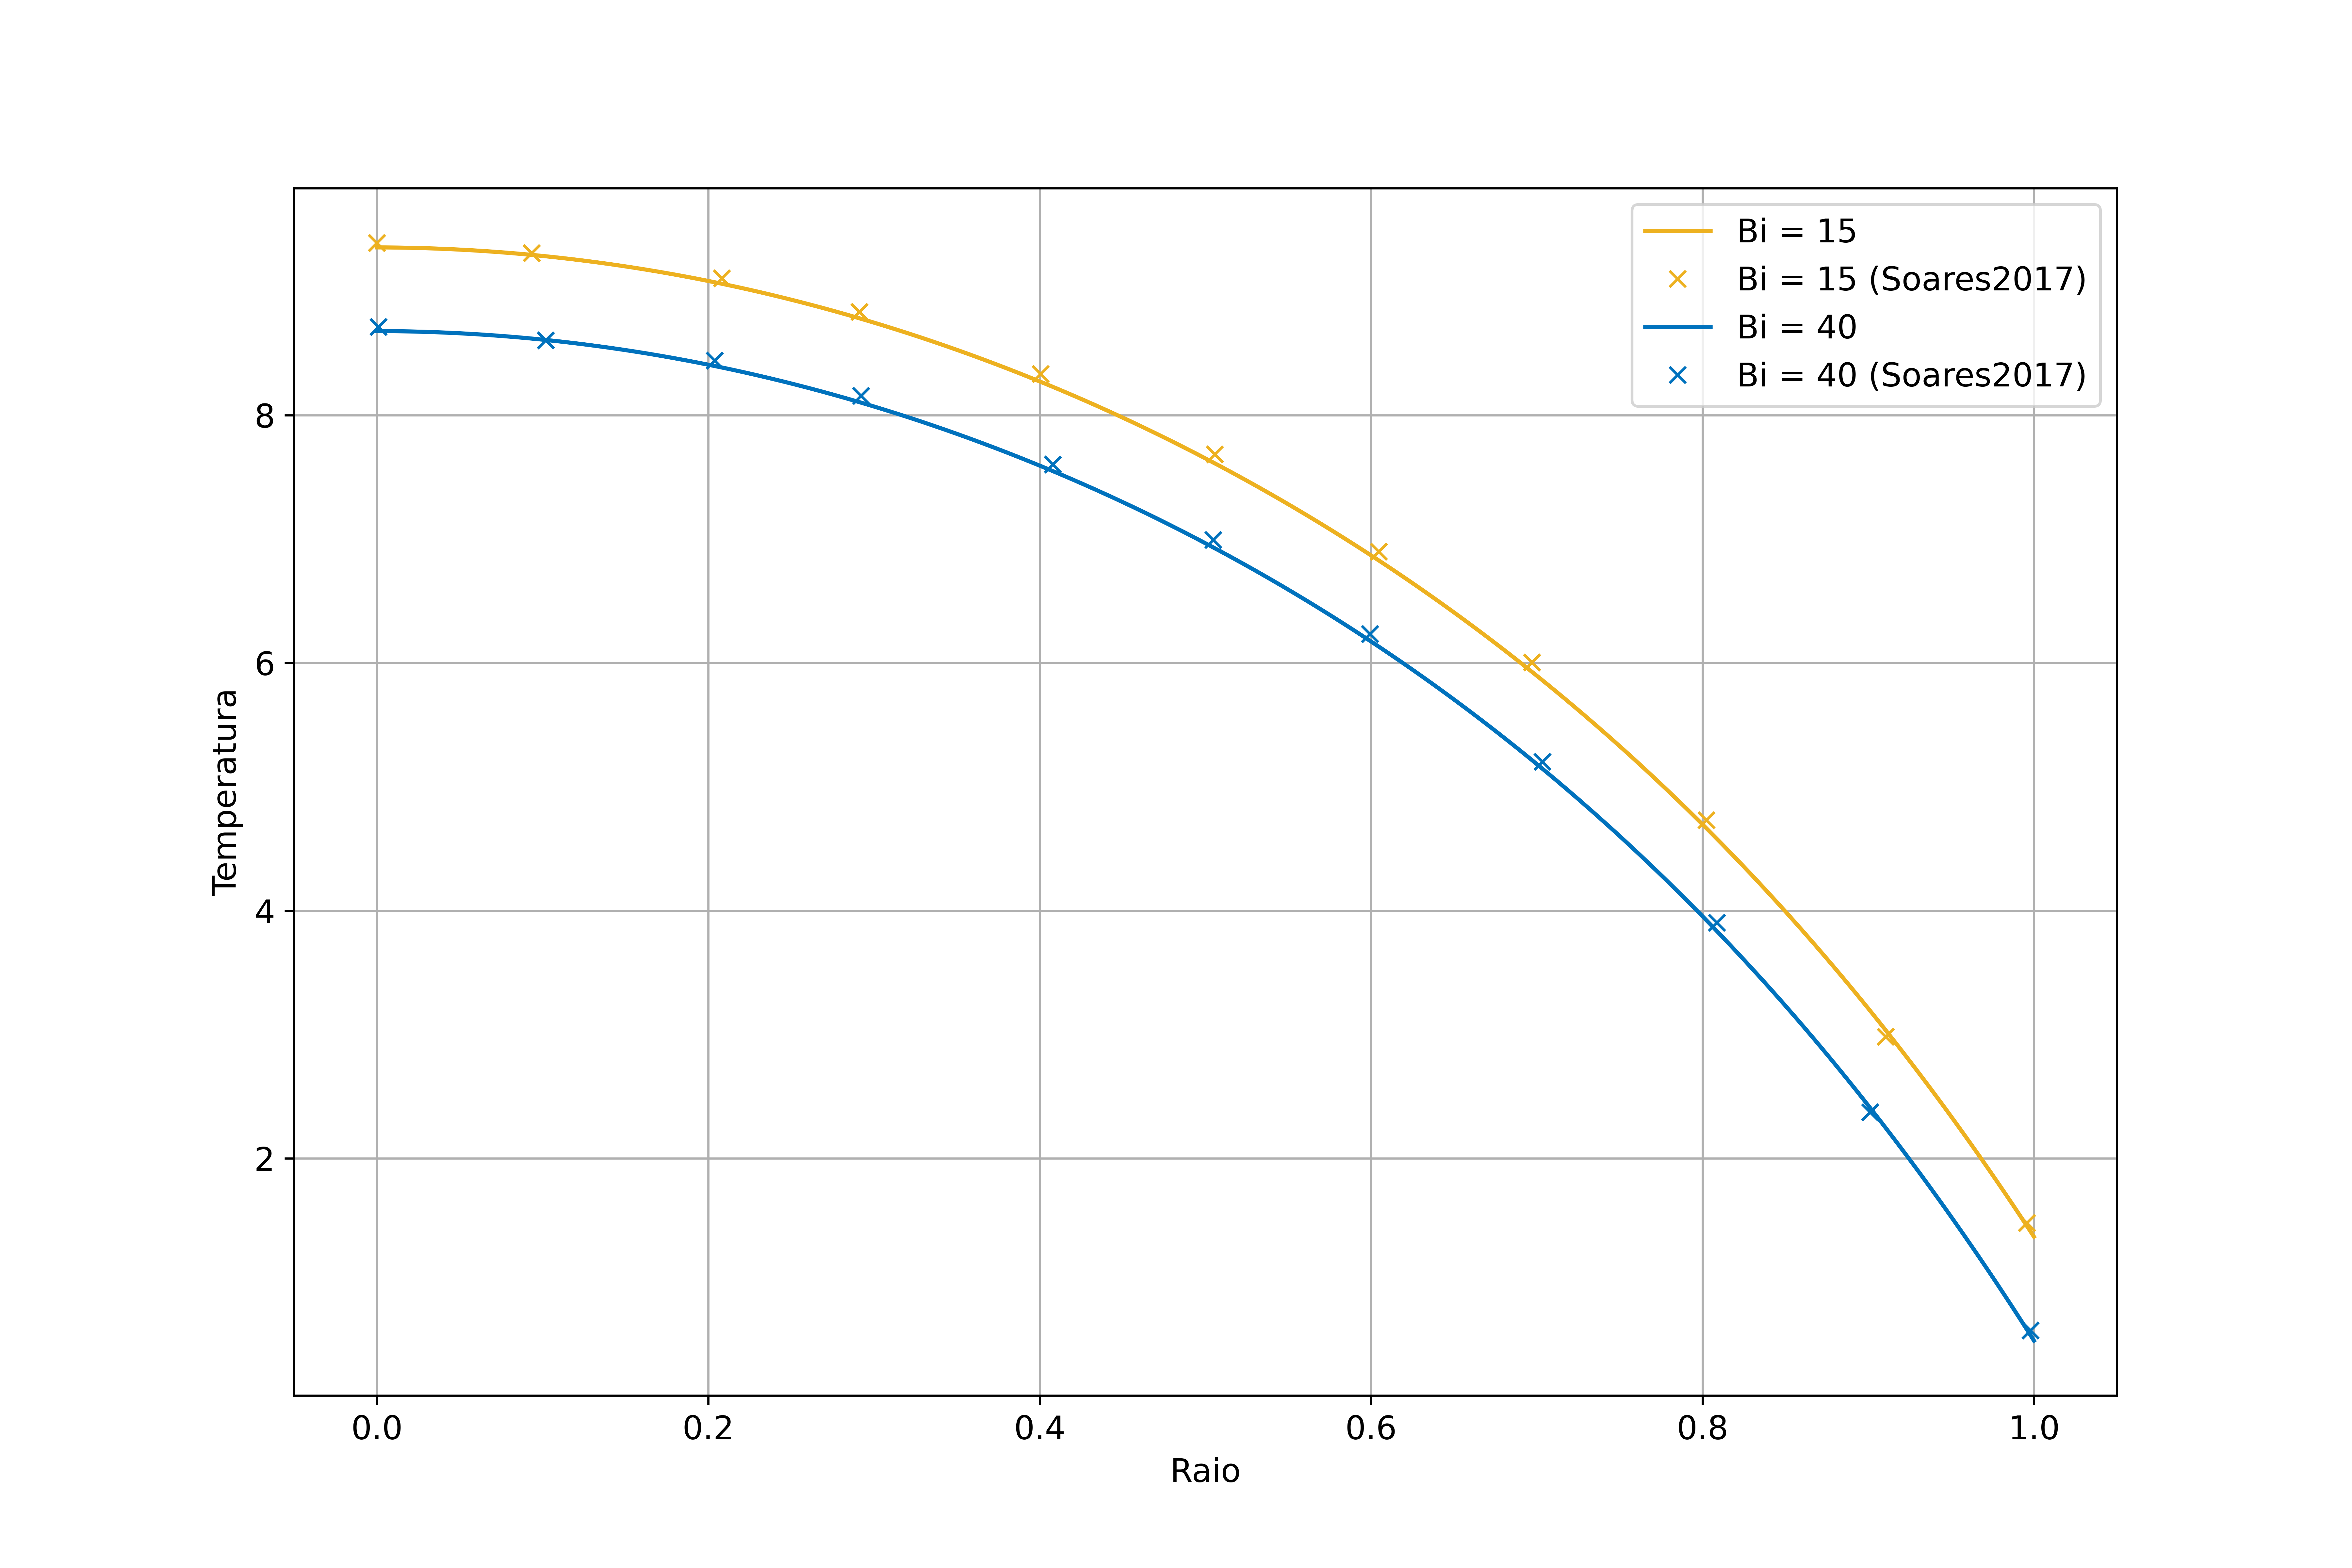
\includegraphics[scale=0.7]{figures/results/Fig15.png}
    \source{Autor, 2023.}
    \label{fig:influence_of_Biot_on_fourth_heat_generation}
\end{figure}

Por fim, buscou-se estudar a influência do número de Biot nos perfis de temperatura. Através da Figura \ref{fig:influence_of_Biot_on_fourth_heat_generation} pode-se observar que com o aumento do número de Biot, houve um descréscimo dos valores de temperatura, algo esperado devido a interpretação do mesmo (razão entre o coeficiente de transferência convectiva de calor na superfície e a condutância específica).
